\chapter{Sprint 4: Event Participation}

\section{Introduction}
In this sprint, we will be focusing on the event participation feature. We will be implementing features
that will allow ODC coordinators to create events and allow users to participate in them.

\section{Sprint Backlog}
As usual, we will be using the sprint backlog to keep track of the tasks that we need to complete in this sprint.
The sprint backlog for this sprint is shown in Table \ref{table:sprint4_backlog}.

\begin{longtable}{|p{2cm}|p{5cm}|p{2cm}|p{5cm}|}
  \hline
  \rowcolor{green!20} \textbf{User Story ID} & \textbf{User Story}                                            & \textbf{Task ID} & \textbf{Task Description}                                           \\ \hline
  \endfirsthead
  \hline
  \rowcolor{green!20} \textbf{User Story ID} & \textbf{User Story}                                            & \textbf{Task ID} & \textbf{Task Description}                                           \\ \hline
  \endhead
  \hline
  % User Story 1
  1                                          & As an ODC Coordinator, I want to be able to create events      & 1.1              & Build user interface for creating events                            \\ \cline{3-4}
                                             &                                                                & 1.2              & Build needed APIs for event creation                                \\ \cline{3-4}
                                             &                                                                & 1.3              & Integrate and test API and user interface for event creation        \\ \hline
  % User Story 2
  2                                          & As an ODC Coordinator, I want to be able to view all events    & 2.1              & Build user interface for viewing all events                         \\ \cline{3-4}
                                             &                                                                & 2.2              & Build needed APIs for retrieving event list                         \\ \cline{3-4}
                                             &                                                                & 2.3              & Integrate and test API and user interface for viewing events        \\ \hline
  % User Story 3
  3                                          & As a Participant, I want to view event details                 & 3.1              & Build user interface for viewing event details                      \\ \cline{3-4}
                                             &                                                                & 3.2              & Build needed APIs for retrieving event details                      \\ \cline{3-4}
                                             &                                                                & 3.3              & Integrate and test API and user interface for viewing event details \\ \hline
  % User Story 4
  4                                          & As a Participant, I want to be able to participate in an event & 4.1              & Build user interface for event participation                        \\ \cline{3-4}
                                             &                                                                & 4.2              & Build needed APIs for event participation                           \\ \cline{3-4}
                                             &                                                                & 4.3              & Integrate and test API and user interface for event participation   \\ \hline

  5                                          & As a Participant, I want to be submit my tests                 & 4.1              & Build user interface for test submit                                \\ \cline{3-4}
                                             &                                                                & 4.2              & Build needed APIs for test submit                                   \\ \cline{3-4}
                                             &                                                                & 4.3              & Integrate and test API and user interface for test submit           \\ \hline
  \caption{Sprint Backlog}
\end{longtable}

\section{Functional Requirements}
\subsection{Use Case Diagram}
The following use case diagram \ref{fig:event_participation_use_case} illustrates the use cases
that we need to cover in this sprint.

\begin{figure}[h!]
  \centering
  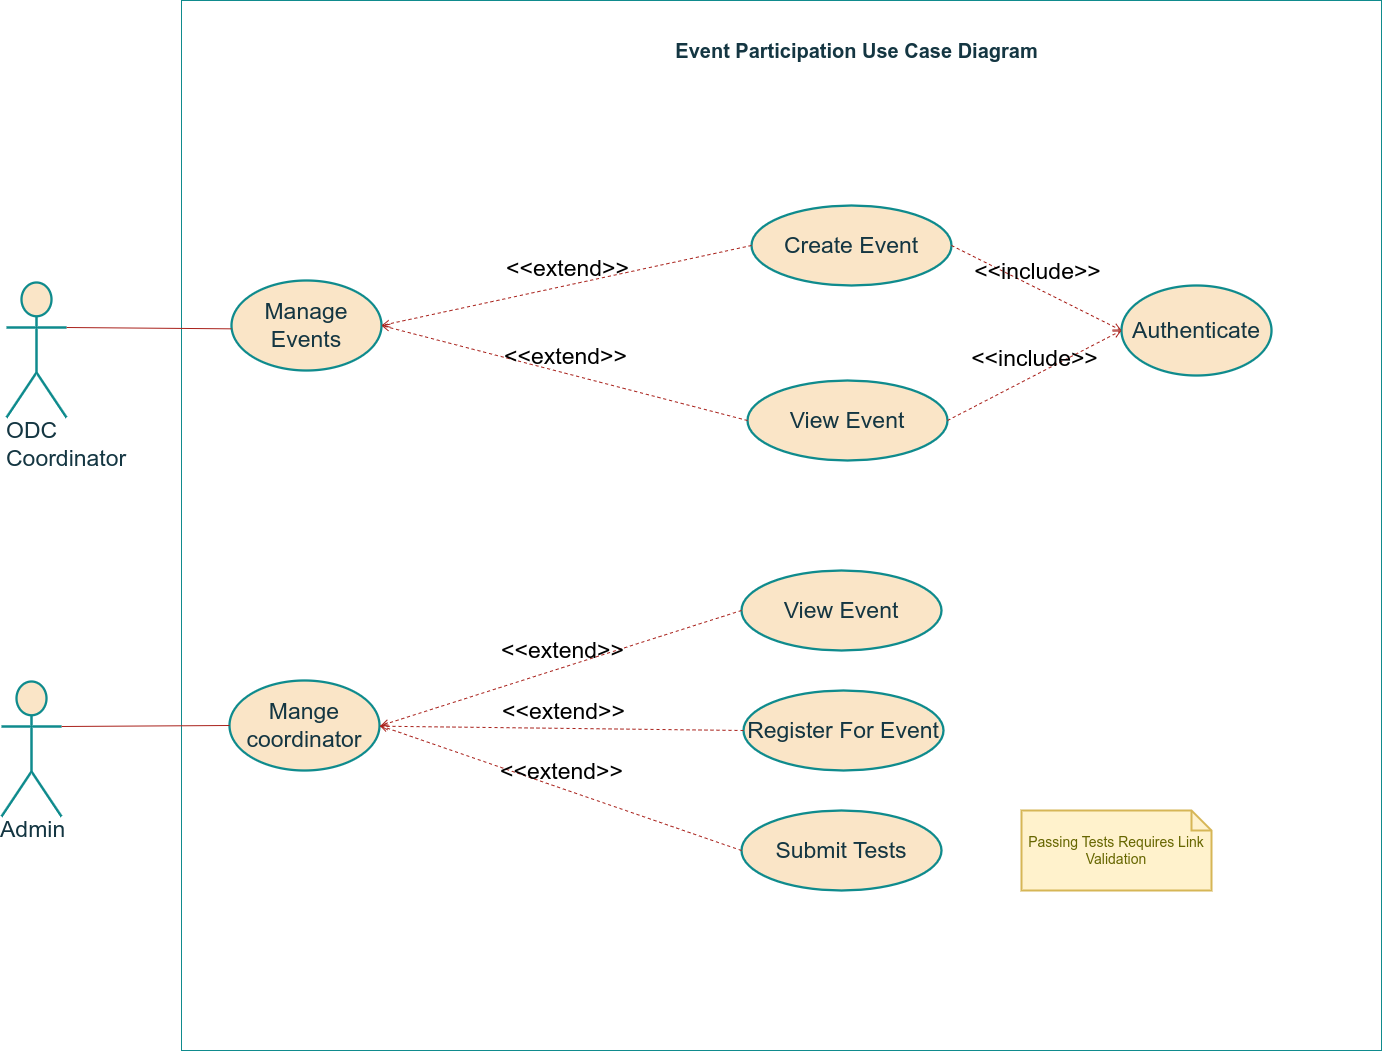
\includegraphics[width=0.8\textwidth]{images/EventParticipationUseCase.png}
  \caption{Event Participation Use Case Diagram}\label{fig:event_participation_use_case}
\end{figure}

One of the crucial use cases that we need to implement is the event registration use case.
This will allow participant to register for an event and therefor engage them with ODC activities.

The table \ref{tab:Textual_Description_of_the_Use_Case_Register_for_an_Event} provides a textual description of the use case `register for an event`.

\begin{table}[h]
  \centering
  \renewcommand{\arraystretch}{1.5}
  \begin{tabular}{|p{3cm}|p{12cm}|}
    \hline
    \rowcolor{green!20} \textbf{Use Case} & Register for an Event                                                                                                            \\
    \hline
    \textbf{Actor}                        & Participant                                                                                                                      \\
    \hline
    \textbf{Brief Description}            & The Participant registers for an event by providing necessary details and confirming the registration.                           \\
    \hline
    \textbf{Pre-condition}                & The Participant must be logged into the system and the event must be available for registration.                                 \\
    \hline
    \textbf{Post-condition}               & The Participant is successfully registered for the event and receives a notification.                                            \\
    \hline
    \textbf{Main Scenario}                & \begin{tabular}[l]{@{}l@{}}
                                              1. The Participant navigates to the event page.                    \\
                                              2. The Participant clicks on the "Register" button.                \\
                                              3. The system prompts the Participant to confirm the registration. \\
                                              4. The Participant confirms the registration.                      \\
                                              5. The system processes the registration and updates the database. \\
                                              6. The system notifies the Participant of the successful registration.
                                            \end{tabular}                                                            \\
    \hline
    \textbf{Exception Scenario}           & \begin{tabular}[l]{@{}l@{}}
                                              1.1 The event is no longer available for registration:                           \\
                                              1.1.1 The system displays a message indicating that the event is full or closed. \\
                                              4.1 The registration process fails due to a system error:                        \\
                                              4.1.1 The system displays an error message and prompts the Participant           \\ to try again later.
                                            \end{tabular}                           \\
    \hline
    \textbf{Extension}                    & If the Participant has already registered for the event, the system will display a message indicating the existing registration. \\
    \hline
  \end{tabular}
  \caption{Textual Description of the Use Case `Register for an Event`}\label{tab:Textual_Description_of_the_Use_Case_Register_for_an_Event}
\end{table}


After being able to register for an event the participant can later participate and submit their tests.
For this we need to better understand this use case to deliver the best experience for the participant.

The table \ref{tab:Textual_Description_of_the_Use_Case_Submit_Test} provides a textual description of the use case `Submit Test`.

\begin{table}[h!]
  \centering
  \renewcommand{\arraystretch}{1.5}
  \begin{tabular}{|p{3cm}|p{12cm}|}
    \hline
    \rowcolor{green!20} \textbf{Use Case} & Submit Test                                                                                  \\
    \hline
    \textbf{Actor}                        & Participant                                                                                  \\
    \hline
    \textbf{Brief Description}            & The Participant submits a completed test to the system for evaluation.                       \\
    \hline
    \textbf{Pre-condition}                & The Participant must be logged into the system and have an active test session.              \\
    \hline
    \textbf{Post-condition}               & The test is successfully submitted, and the Participant receives a notification.             \\
    \hline
    \textbf{Main Scenario}                & \begin{tabular}[l]{@{}l@{}}
                                              1. The Participant completes the test questions.                 \\
                                              2. The Participant clicks on the "Submit Test" button.           \\
                                              3. The system validates the test submission.                     \\
                                              4. The system processes the submission and updates the database. \\
                                              6. The system displays next test.
                                            \end{tabular}                             \\
    \hline
    \textbf{Exception Scenario}           & \begin{tabular}[l]{@{}l@{}}
                                              3.1 The test submission fails due to a system error:                      \\
                                              3.1.1 The system displays an error message and prompts the Participant to \\ try again later.
                                            \end{tabular} \\
    \hline
  \end{tabular}
  \caption{Textual Description of the Use Case `Submit Test`}\label{tab:Textual_Description_of_the_Use_Case_Submit_Test}
\end{table}


\section{Analysis and Design}
Now that we have identified the tasks that need to be completed in this sprint, we will proceed with the analysis and design phase.
We will start by analyzing the use cases for the event participation feature and then move on to designing the system.

Once our participants registered for the event, we need to figure out how to notify them when the event is about to start.
To do so we decided to implement a notification system that relies on a cron job that will run every 5 minutes to check for any upcoming events.
if an event is about to start, the system will send an email to each participant registered for the event. The event link will contain a special
token that will allow the participant to join the event directly.

The token will be also used to identify the participant when saving the test submission result

In the following sequence diagram \ref{fig:fetch_list_of_tests} we illustrate the sequence of actions that will happen
when the participant opens the event participation page.

\begin{figure}[h!]
  \centering
  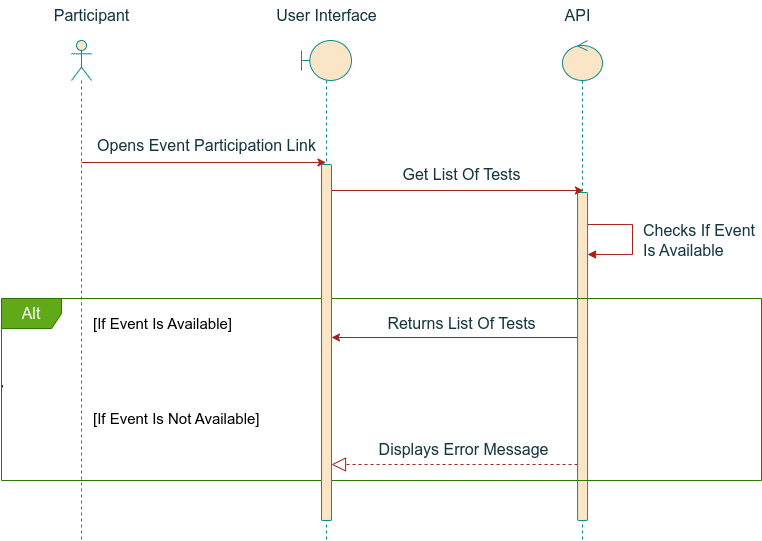
\includegraphics[width=0.8\textwidth]{images/sequenceChecksIfEventIsAvailable.png}
  \caption{Fetch List Of Tests}\label{fig:fetch_list_of_tests}
\end{figure}

Moving to the test submission feature Where the participant will be able to submit their test answers to the system for evaluation.
At the evaluation stage, the system will compare the participant's answers with the correct answers and calculate the score.
and then will save it to the database.

Later on we can use the data to calculate the participant's total score and rank the participants accordingly.

The sequence diagram in figure \ref{fig:event_participation_class_diagram} illustrates
how the system will handle the test submission process.

\begin{figure}[h!]
  \centering
  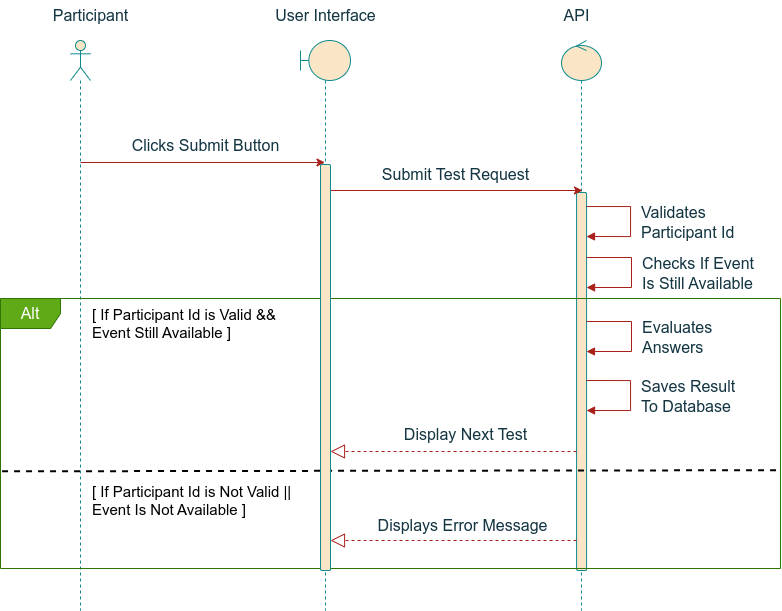
\includegraphics[width=0.8\textwidth]{images/sequencePassTest.png}
  \caption{Event Participation Class Diagram}\label{fig:event_participation_class_diagram}
\end{figure}


\section{Implementation}

In this section we will showcase some of the interfaces that we have implemented during the sprint.

\subsection{Event Creation Interface}
The event creation interface allows ODC coordinators to create events. The interface is shown in figure \ref{fig:event_creation_interface}.

\begin{sidewaysfigure}[h!]
  \centering
  \setlength\fboxsep{0pt} % Adjusts the separation between the image and the border
  \setlength\fboxrule{2pt} % Adjusts the thickness of the border
  \fcolorbox{orange}{white}{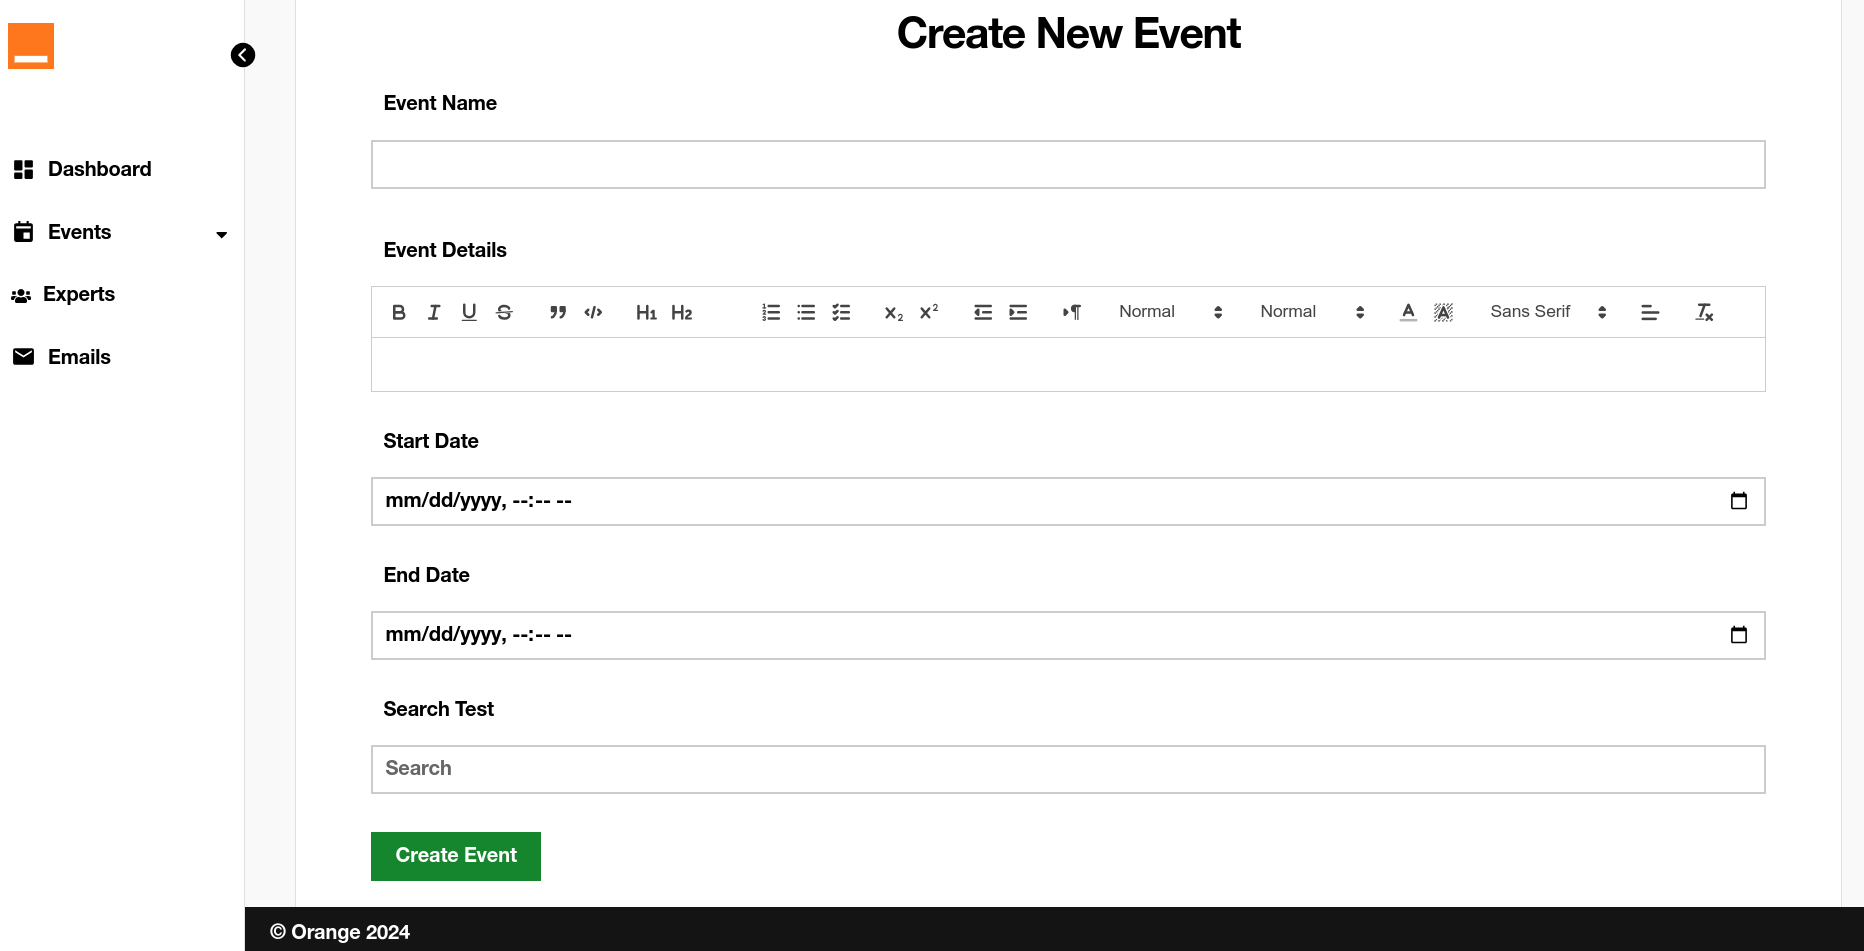
\includegraphics[width=0.8\paperheight, height=0.6\paperwidth]{images/eventCreation.png}}
  \caption{Event Creation Page}\label{fig:event_creation_interface}
\end{sidewaysfigure}

\subsection{Event Details Page}
The figure \ref{fig:event_details_page} show the page where the participant will be able to view the event content
such as the event description, the event date and time.

\begin{sidewaysfigure}[h!]
  \centering
  \setlength\fboxsep{0pt} % Adjusts the separation between the image and the border
  \setlength\fboxrule{2pt} % Adjusts the thickness of the border
  \fcolorbox{orange}{white}{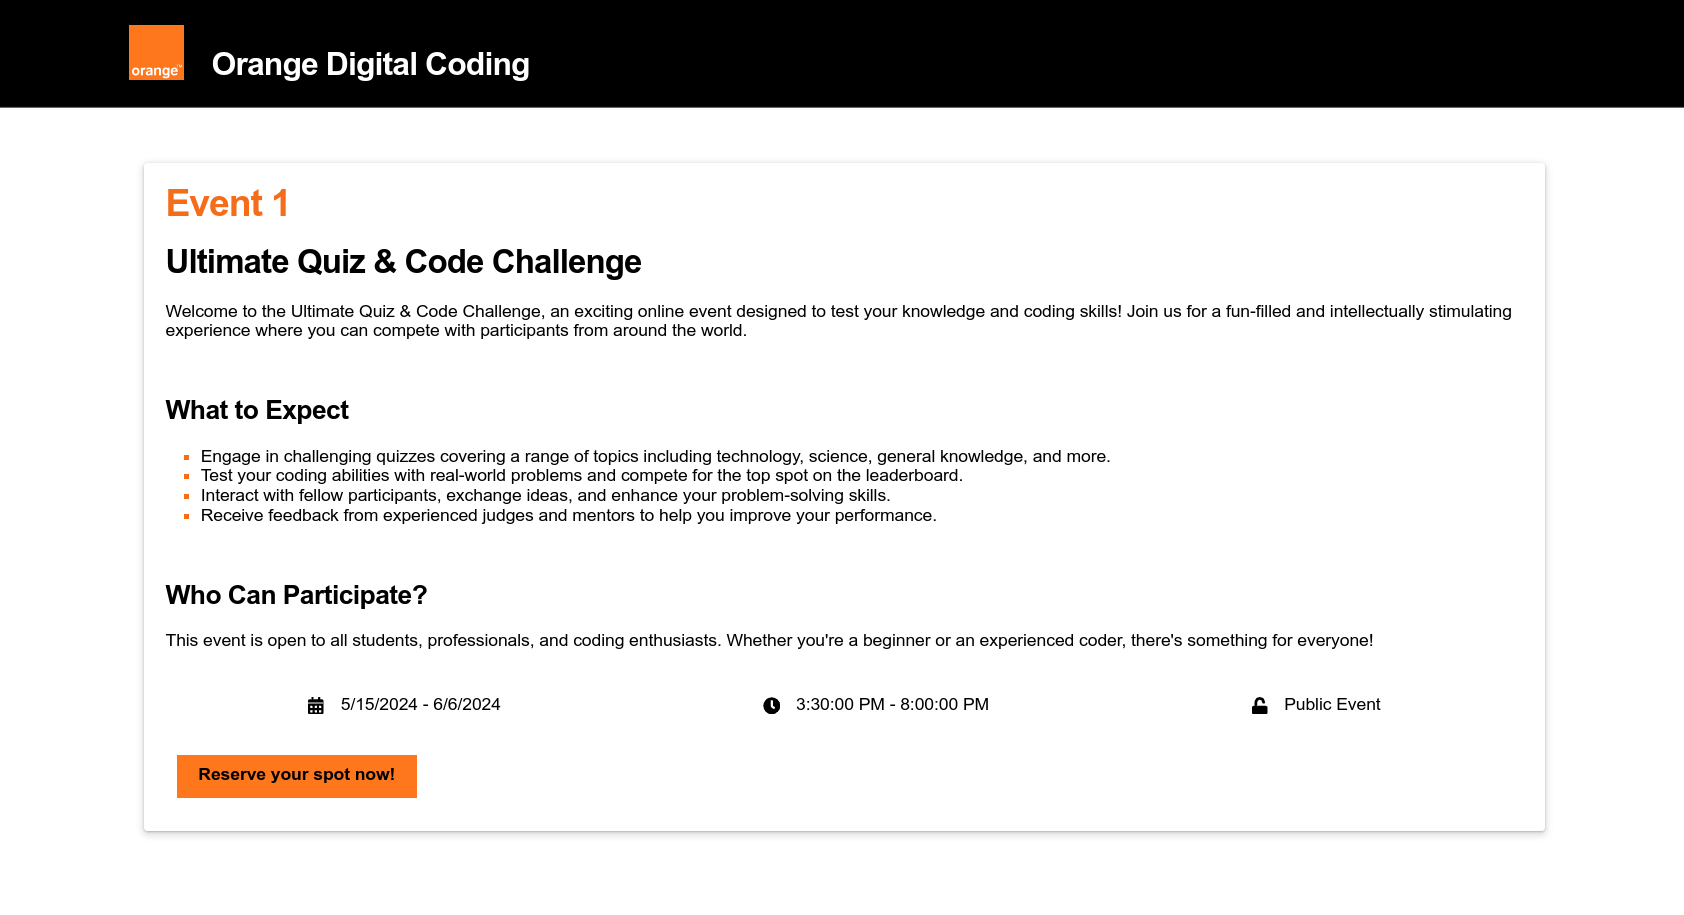
\includegraphics[width=0.8\paperheight, height=0.6\paperwidth]{images/eventDetails.png}}
  \caption{Event Details Page}\label{fig:event_details_page}
\end{sidewaysfigure}


\subsection{Event Registration Form}
The participant can use the following form illustrated in figure \ref{fig:event_registration_page} to register for an event. They can trigger
the registration process by clicking on the `Register` button.

\begin{sidewaysfigure}[h!]
  \centering
  \setlength\fboxsep{0pt} % Adjusts the separation between the image and the border
  \setlength\fboxrule{2pt} % Adjusts the thickness of the border
  \fcolorbox{orange}{white}{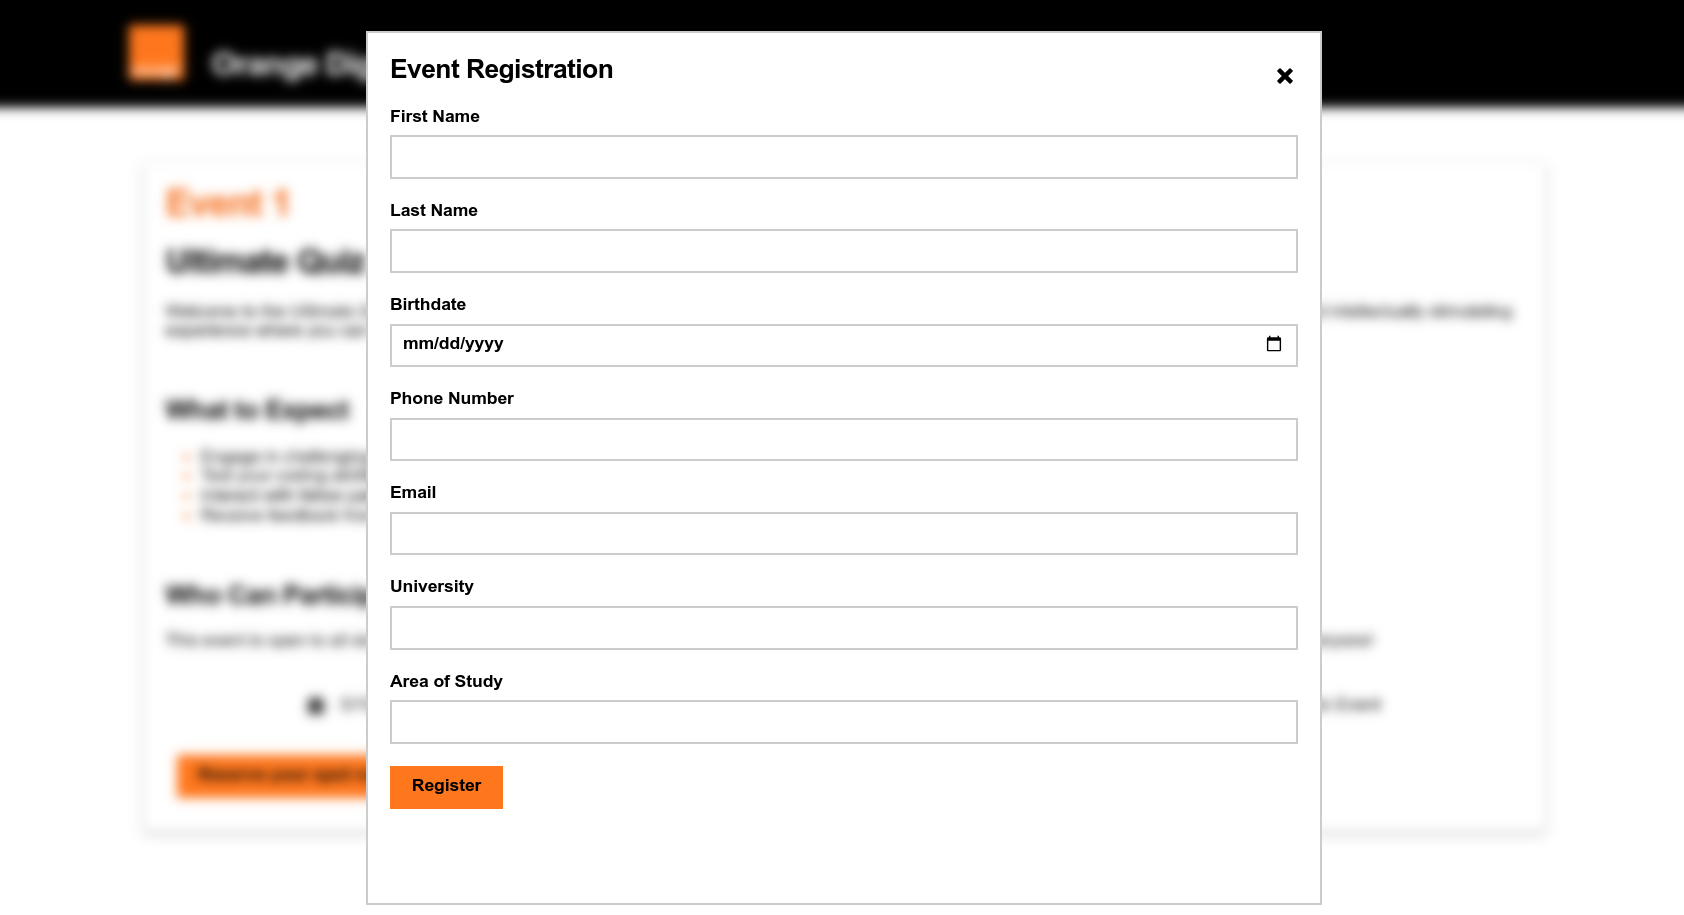
\includegraphics[width=0.8\paperheight, height=0.6\paperwidth]{images/eventRegistration.png}}
  \caption{Event Registration Page}\label{fig:event_registration_page}
\end{sidewaysfigure}


\subsection{Quiz Submission Page}
After the choosing the right quiz answer the participant will be able to submit their
answers to the system for evaluation using The interface is shown in figure \ref{fig:submit_quiz}.

\begin{sidewaysfigure}[h!]
  \centering
  \setlength\fboxsep{0pt} % Adjusts the separation between the image and the border
  \setlength\fboxrule{2pt} % Adjusts the thickness of the border
  \fcolorbox{orange}{white}{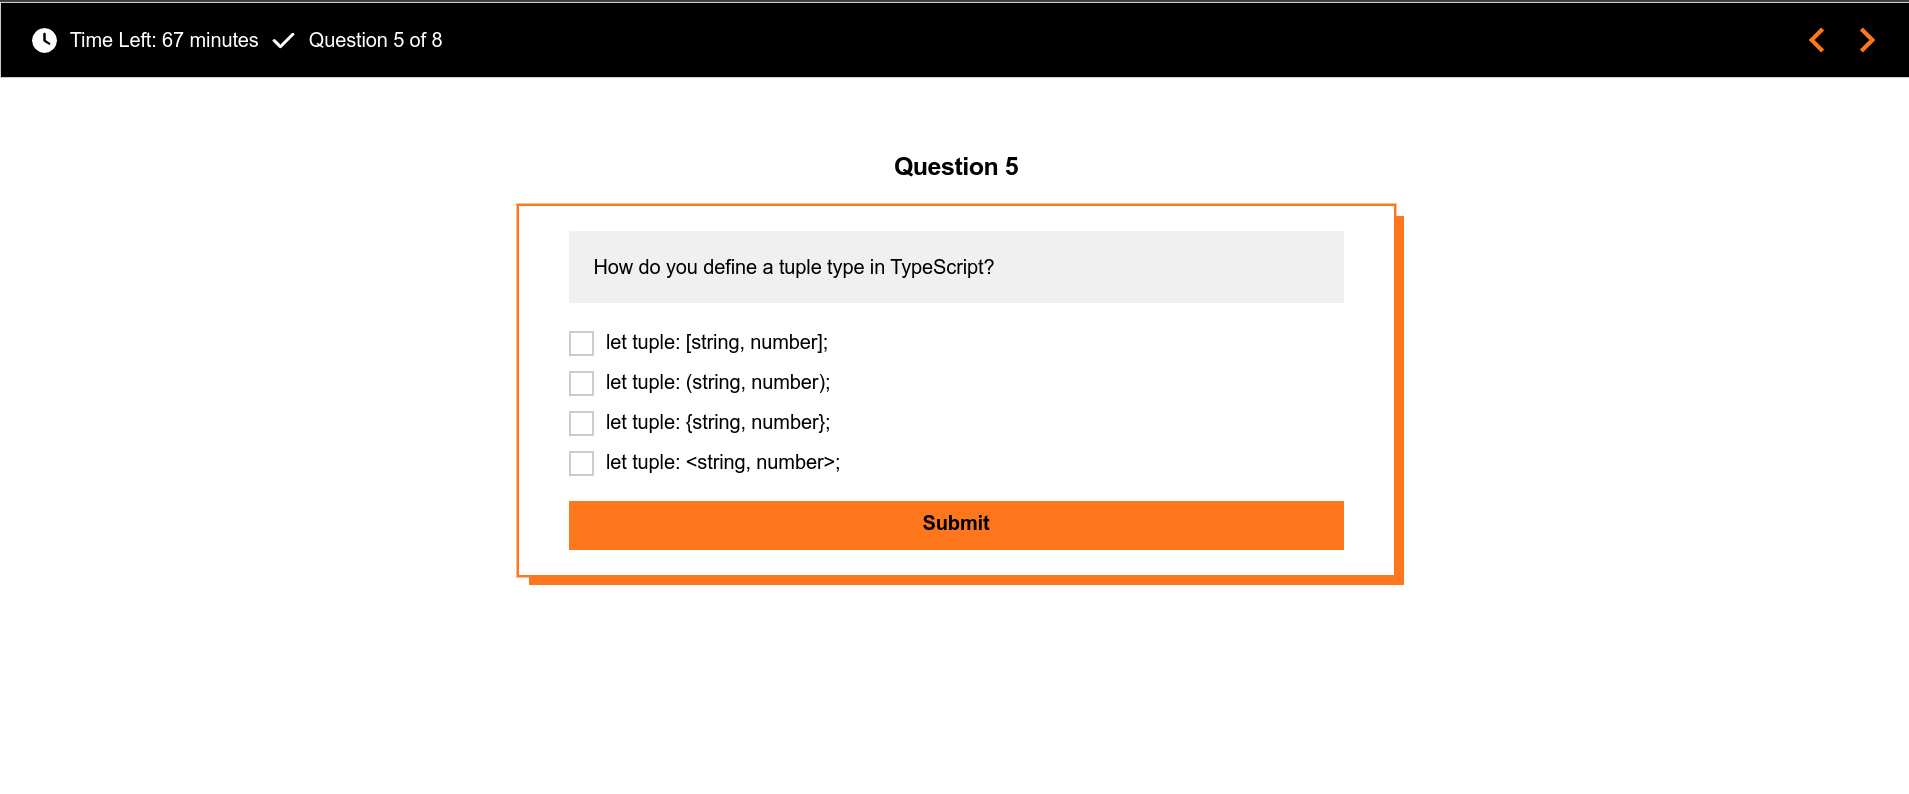
\includegraphics[width=0.8\paperheight, height=0.6\paperwidth]{images/quizTestEvent.png}}
  \caption{Submit Quiz Page}\label{fig:submit_quiz}
\end{sidewaysfigure}


\subsection{Problem Submission Page}
After writing the code solution the participant will be able to submit their
answers to the system for evaluation as shown in figure \ref{Problem Submit Page}.


\begin{sidewaysfigure}[h!]
  \centering
  \setlength\fboxsep{0pt} % Adjusts the separation between the image and the border
  \setlength\fboxrule{2pt} % Adjusts the thickness of the border
  \fcolorbox{orange}{white}{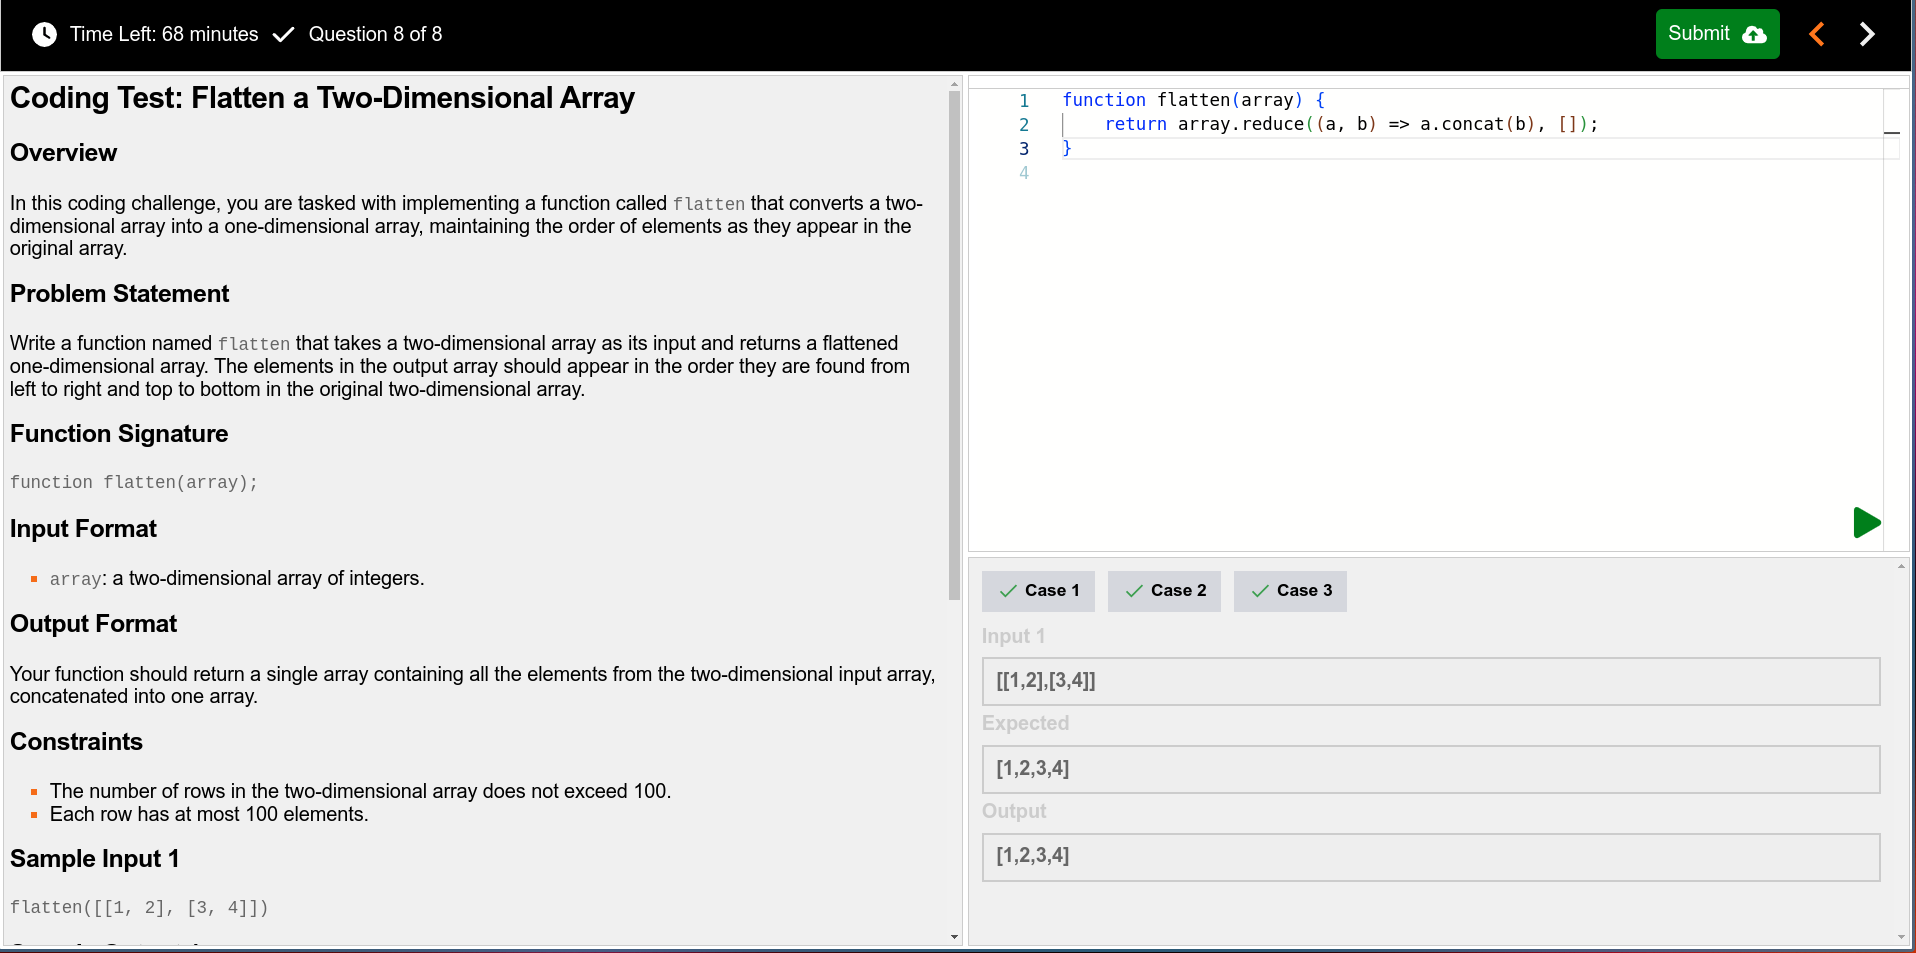
\includegraphics[width=0.8\paperheight, height=0.6\paperwidth]{images/problemTestEvent.png}}
  \caption{Problem Submit Page}\label{Problem Submit Page}
\end{sidewaysfigure}
